\section{The noise floor}\label{sec:noise}

Realistic noise raises the Mackey--Glass error of the spectral-phase mask from $1.8\times10^{-6}$ to $3.3\times10^{-4}$, a factor of
about 180 (Table~\ref{tab:encodings}). Section~\ref{sec:mechanism} showed that the mask operates in the coherently seeded regime, so
its error comes from noise, not from non-reproducible dynamics. This section separates the five noise sources to answer three
questions: which of them set the floor; whether a more nonlinear material or more power lowers it; and whether it can be removed
in the readout. The answer: about half of the floor comes from detuning jitter and half from shot noise. The first half does not
depend on the photon number; the second falls with more photons, but then the first half quickly dominates, so neither
Si$_3$N$_4$ nor more power helps much. A linear readout cannot remove the jitter even when it knows the exact jitter sequence, so it
has to be suppressed at the source, which sets a requirement on the laser linewidth.

\subsection{Breakdown}\label{sec:breakdown}

To separate the detectors from the noise inside the device, we first assume ideal detectors (no electronic noise, shot noise only),
choose the best of 256 random operating points with the protocol of Section~\ref{sec:protocol}, and switch on one noise source at a
time at that point (Fig.~\ref{fig:noise}a). The point uses $23~\mathrm{mW}$ in total, a loaded $Q$ of $6\times10^{6}$, and about
$170~\mu\mathrm{W}$ per line at the detector, i.e.\ about $1.3\times10^{6}$ photons per symbol.
Its error without noise is $1.3\times10^{-5}$. With only the laser intensity noise it is $1.9\times10^{-5}$, nearly unchanged; with
only the intracavity vacuum noise $2.5\times10^{-5}$; with only the detuning jitter $5.7\times10^{-5}$; with only shot noise
$6.8\times10^{-5}$. The three optical sources together give $7.8\times10^{-5}$, and adding shot noise gives $1.5\times10^{-4}$.
The floor with ideal detectors is therefore about $1.3\times10^{-4}$ (after re-selecting among 256 points), about half from
detuning jitter and half from shot noise, with the vacuum noise secondary and the laser intensity noise negligible.

With realistic PIN detectors ($0.3~\mu\mathrm{W}$ electronic noise per line) the same procedure selects a point at
$3.4\times10^{-4}$, another factor of about 2.5. The effect of the detectors shows most clearly in an earlier, smaller search (32
candidates per encoding, selection on a single run): with all noise on and detector noise of $0.03$, $0.1$, $0.3$ and
$0.6~\mu\mathrm{W}$ the error is $2.7\times10^{-4}$, $4.1\times10^{-4}$, $1.0\times10^{-3}$ and $2.2\times10^{-3}$, roughly linear in
the detector noise above $0.1~\mu\mathrm{W}$; an optical amplifier with $10~\mathrm{dB}$ or $20~\mathrm{dB}$ gain and a
$5~\mathrm{dB}$ noise figure in front of the $0.3~\mu\mathrm{W}$ detectors brings it to $3.3\times10^{-4}$ and $3.1\times10^{-4}$,
close to the $2.4\times10^{-4}$ with optical and shot noise only. These numbers cannot be compared directly with
Table~\ref{tab:encodings} (fewer candidates, different selection); we use them only for the trend: electronic detector noise can be
removed with an optical amplifier, and what remains is the floor above.

\begin{figure}[htbp]
\centering
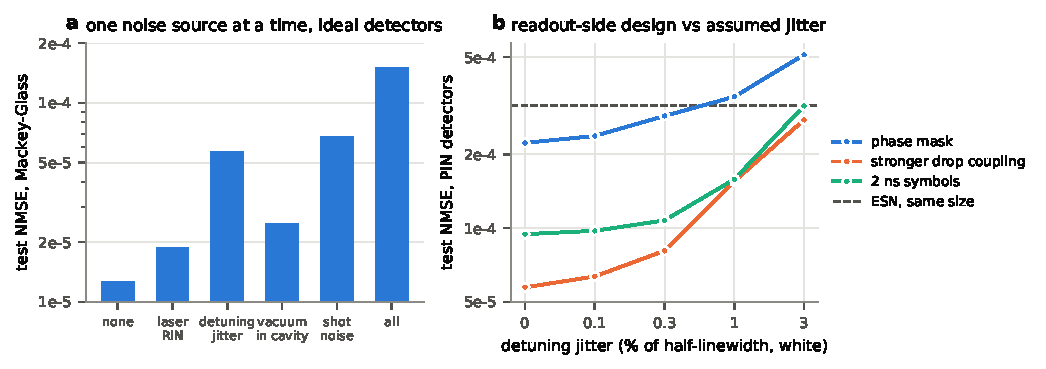
\includegraphics[width=\linewidth]{fig6_noise}
\caption{Noise and readout-side design (Mackey--Glass).
(a) Test error at the best of 256 operating points with ideal detectors, one noise source at a time; ``all'' has the four sources
(laser intensity noise, detuning jitter, intracavity vacuum noise, shot noise) on together.
(b) Test error, with the operating point re-selected at each level, against the assumed detuning jitter (rms per symbol in percent
of the half-linewidth, correlation $e^{-1}$ between neighbouring symbols; the horizontal axis is categorical), PIN detectors: plain
spectral-phase mask, stronger drop coupling, $2~\mathrm{ns}$ symbols; dashed: ESN with the same readout dimension (input noise
$3\times10^{-3}$, one random reservoir). The top axis gives the intrinsic laser linewidth that produces the same jitter at the
stronger-drop-coupling point ($Q=1.9\times10^{6}$, $1~\mathrm{ns}$, Eq.~\eqref{eq:linewidth}); for the $2~\mathrm{ns}$ point
($Q=5\times10^{6}$) the linewidths are about 0.3 times these.}
\label{fig:noise}
\end{figure}

\subsection{Neither a more nonlinear material nor more power lowers the floor}\label{sec:platform}

Shot noise can be reduced with more photons; detuning jitter cannot, because it is defined relative to the resonance linewidth and
does not depend on how many photons are in the cavity. We changed the photon number in two ways, re-searching 256 operating points
each time (ideal detectors):
\begin{itemize}
\item a Si$_3$N$_4$ ring (nonlinear coefficient about 60 times that of silica, power range scaled with $\gamma L$ so that the
      normalised pump covers the same range): the best point needs only $5~\mathrm{mW}$ and delivers about 8 times fewer photons to
      the detectors, yet the floor is $1.4\times10^{-4}$, the same as silica's $1.3\times10^{-4}$;
\item a silica ring with ten times the power range ($0.1$ to $3~\mathrm{W}$): the floor is $1.5\times10^{-4}$, no improvement. Its best
      point has 4.4 times more photons per line than the point above, but the shot-noise term only falls from $6.8\times10^{-5}$ to
      $5.3\times10^{-5}$, and the jitter term ($5.1\times10^{-5}$) barely changes.
\end{itemize}
The shot-noise term falls much more slowly than the photon number grows, but the two best points also differ in other parameters,
so this is only a rough comparison. A controlled comparison keeps the operating point and the intracavity dynamics fixed and changes
only the number of photons detected per reading (the best single ring, ideal detectors, three series $\times$ six new pairs): with
1, 10 and 100 times the photons the total error is $1.41\times10^{-4}$, $1.21\times10^{-4}$ and $1.16\times10^{-4}$, and
$1.16\times10^{-4}$ without shot noise. The shot-noise term itself does fall with the photon number (about 5 times for 10 times the
photons, about 40 times for 100 times), but the total quickly settles at the level set by the optical noise, mostly detuning jitter.
At this point more power can lower the error by at most about 18\%.
The benefit of Si$_3$N$_4$ is power: the same floor needs about a quarter of the power; but with ordinary detectors fewer photons
reach them and the error rises to $1.1\times10^{-3}$, so it needs better detectors or an optical amplifier.
What does lower the floor is the readout side: stronger drop coupling (more light to the detectors) or $2~\mathrm{ns}$ symbols (longer
integration per reading) bring it to $8.7\times10^{-5}$ and $6.9\times10^{-5}$ with ideal detectors, and $1.55\times10^{-4}$ and
$1.58\times10^{-4}$ with ordinary detectors (Section~\ref{sec:readout}).

\subsection{A linear readout cannot remove the detuning jitter}\label{sec:reference}

If the detuning jitter comes mainly from the frequency noise of the pump laser, all rings on one chip driven by the same laser see
the same jitter. A natural idea is a reference ring without signal that measures this common-mode noise so the readout can subtract
it. We first measure the upper bound of this idea: on the best single ring (stronger drop coupling, $Q=1.9\times10^{6}$,
$178~\mathrm{mW}$) we hand the readout the true jitter sequence of each run (current and previous seven symbols), i.e.\ a noiseless
ideal reference. Over three series with six new pairs each, the plain readout gives $1.60\times10^{-4}$; adding the true jitter
sequence gives $1.58\times10^{-4}$, only 2\% better; also adding the products of the current jitter with the line features (so that
the correction can depend on the state) is slightly worse, $1.65\times10^{-4}$. Switching the jitter itself off, with all other
noise unchanged, gives $5.7\times10^{-5}$, 2.8 times better.

So the jitter is indeed the larger part of the floor, but even when it is known exactly a linear readout cannot remove it.
The reason is that the jitter is not additive noise on the readings: it changes the intracavity detuning, which changes the state of
the whole comb through the nonlinear dynamics and persists over the following symbols; its effect on each line depends on the state
at the time and cannot be subtracted linearly by the readout. A shared reference ring read out linearly therefore does not work. We
did not test nonlinear readouts, or feeding the reference ring's own 31 line features (which are nonlinear functions of the jitter
history) to the readout; these could recover part of the gap, but the jitter is most simply suppressed physically.

\subsection{Requirement on the intrinsic laser linewidth}\label{sec:laser}

The noise model above gives every symbol a detuning jitter of 1\% of the half-linewidth (rms). We now relate it to the laser.
For white frequency noise with Lorentzian linewidth $\Delta\nu$ (one-sided frequency-noise spectrum $S_\nu=\Delta\nu/\pi$), the
variance of the frequency averaged over a symbol time $T$ is $\Delta\nu/(2\pi T)$. In units of the half-linewidth $\nu/(2Q)$, the
relative jitter per symbol $\varepsilon$ and the linewidth are related by
\begin{equation}
\Delta\nu=2\pi T\left(\frac{\varepsilon\,\nu}{2Q}\right)^{2}.
\label{eq:linewidth}
\end{equation}
For the best single ring ($Q=1.9\times10^{6}$, half-linewidth $51~\mathrm{MHz}$, $T=1~\mathrm{ns}$), 1\% jitter corresponds to an
intrinsic linewidth of about $1.6~\mathrm{kHz}$, and 0.3\% and 0.1\% to about $150~\mathrm{Hz}$ and $16~\mathrm{Hz}$; conversely, a
laser with a $100~\mathrm{kHz}$ intrinsic linewidth produces about 8\% jitter. The required linewidth tightens with the square of $Q$
and relaxes with the symbol time: at the $2~\mathrm{ns}$ point of Section~\ref{sec:readout} ($Q=5\times10^{6}$), 1\% corresponds to
about $470~\mathrm{Hz}$.

To test this conversion we generate the jitter directly from a realistic laser frequency-noise spectrum $S_\nu(f)=h_0+h_{-1}/f$, where
$h_0=\Delta\nu/\pi$ is the white frequency noise and $h_{-1}/f$ the flicker noise (semiconductor lasers typically have a corner near
$1~\mathrm{MHz}$); the laser is locked to the resonance, and the suppression by the lock is modelled by a first-order high-pass
$f^{2}/(f^{2}+B^{2})$. A time series is synthesised from the spectrum, averaged within each symbol and divided by the half-linewidth to
give the jitter of each run; all other noise is unchanged. Table~\ref{tab:laser} gives the results.

% generated by experiments/make_table2.py; do not edit by hand
\begin{table}[htbp]
\centering
\caption{The best single ring under real lasers (stronger drop coupling, Mackey--Glass, all other realistic noise unchanged). The detuning jitter is the laser's white frequency noise averaged over each symbol. ``Fixed point'' is the point chosen under the 1\% jitter assumption ($Q=1.9\times10^{6}$); ``re-selected'' repeats the selection of Section~\ref{sec:protocol} under this laser's noise (56 candidates per series binned by $Q$). Three series $\times$ six new pairs. The two columns use different noise realisations; the same point differs by about 9\% between them.}
\label{tab:laser}
\small
\begin{tabular}{p{4.2cm}cccc}
\toprule
intrinsic linewidth & jitter/symbol & fixed point & re-selected & re-selected $Q$ \\
\midrule
100~Hz & 0.25\% & $6.7\times10^{-5}$ & -- & -- \\
1.6~kHz & 1.00\% & $1.3\times10^{-4}$ & $1.2\times10^{-4}$ & $1.9\times10^{6}$ \\
16~kHz & 3.15\% & $3.1\times10^{-4}$ & $2.9\times10^{-4}$ & $1.9\times10^{6}$ \\
100~kHz & 7.88\% & $8.1\times10^{-4}$ & $6.4\times10^{-4}$ & $1.9\times10^{6}$, $2.5\times10^{6}$ \\
1~MHz & 24.92\% & $5.2\times10^{-3}$ & $1.6\times10^{-3}$ & $1.2\times10^{6}$ \\
\midrule
100~kHz, flicker noise (1~MHz corner) and 1~MHz lock & 7.92\% & $8.3\times10^{-4}$ & -- & -- \\
1.6~kHz, flicker noise (10~MHz corner), no lock & 1.10\% & $1.8\times10^{-4}$ & -- & -- \\
\bottomrule
\end{tabular}
\end{table}


Table~\ref{tab:laser} shows four things. First, at nanosecond symbols what matters is the intrinsic (white-noise) linewidth: a
$1~\mathrm{ns}$ symbol corresponds to a bandwidth of about $500~\mathrm{MHz}$, almost entirely occupied by white frequency noise,
while the flicker noise is concentrated at low frequencies; adding flicker noise with a $1~\mathrm{MHz}$ corner and a
$1~\mathrm{MHz}$ lock leaves the $100~\mathrm{kHz}$ row nearly unchanged, and only very strong flicker noise ($10~\mathrm{MHz}$
corner) without any lock moves the $1.6~\mathrm{kHz}$ row from $1.3\times10^{-4}$ to $1.8\times10^{-4}$.
Second, our 1\% jitter model (correlation $e^{-1}$ between neighbouring symbols) gives $1.60\times10^{-4}$ at this point, about 25\%
more pessimistic than white frequency noise of the same rms ($1.27\times10^{-4}$), so at this point the main results are slightly
conservative. (The same point evaluated with other noise realisations gives $1.5$ to $1.6\times10^{-4}$; we use $1.55\times10^{-4}$
from Section~\ref{sec:readout} as its reference value.)
Third, changing the operating point does not avoid the requirement: at $1.6~\mathrm{kHz}$ and $16~\mathrm{kHz}$ re-selection returns
the original point; at $100~\mathrm{kHz}$ two series move to a point with $Q=2.5\times10^{6}$ and the error improves by about 1.3
times, more than the 9\% spread of one point between noise realisations but still modest; only at $1~\mathrm{MHz}$ does the choice
move clearly to lower $Q$ ($1.2\times10^{6}$), improving the error 3.3 times, yet the lowest $Q$ among the candidates (about
$5\times10^{5}$) is never chosen, because low-$Q$ points have weak nonlinearity and memory, which cancels the benefit of smaller
jitter.
Fourth, the position relative to software: the 31-node ESN with the same readout dimension and input noise $3\times10^{-3}$ reaches
$1.9\times10^{-4}$ (three reservoirs) to $3.2\times10^{-4}$ (one reservoir); by log interpolation of Table~\ref{tab:laser} the
intrinsic linewidth must be below about $5$ to $17~\mathrm{kHz}$ for the best single ring not to lose to it. Against
$1.9\times10^{-4}$, a $100~\mathrm{kHz}$ laser makes the ring about 4 times worse than the ESN, and a $1~\mathrm{MHz}$ laser about 8
times worse even after re-selection.

This gives the second design rule: \emph{half of the error floor is set by the laser's frequency noise relative to the resonance; a
linear readout cannot remove it and another operating point does not avoid it, so it calls for a narrow-linewidth source}.
For our device ($Q\sim2\times10^{6}$, $1~\mathrm{GBd}$) the intrinsic laser linewidth should be below a few kilohertz.
Self-injection locking of a laser to a microresonator is a known way to narrow semiconductor lasers by orders of
magnitude~\cite{shen2020,jin2021}: for example, self-injection locking an ordinary DFB laser to a silicon-nitride resonator with
$Q>2.6\times10^{8}$ suppresses its frequency noise by about five orders of magnitude and reaches a short-term linewidth of about
$1.2~\mathrm{Hz}$~\cite{jin2021}, far below the few kilohertz required here.
Thermorefractive noise of the ring itself is not included; it is mostly at low frequencies and is expected to matter little on
nanosecond scales after locking, but this needs a separate check.
